\documentclass{article}
\usepackage[utf8]{inputenc}
\usepackage{fullpage}
\usepackage{times}
\usepackage[normalem]{ulem}
\usepackage{fancyhdr,graphicx,amsmath,amssymb, mathtools, scrextend, titlesec, enumitem}
\usepackage[ruled,vlined]{algorithm2e} 
\usepackage{float}
\include{pythonlisting}

\title{t-SNE for Visualizing High-Dimensional Data}
\author{Sarah Mansfield, Emre Yurtbay }
\date{April 27, 2021}

\begin{document}

\maketitle

\begin{center}
GitHub repository: https://github.com/sarahmansfield/t-SNE-py
\end{center}

\section*{Abstract}

We investigate the use of the dimensionality reduction technique called t-distributed stochastic neighbor embedding or t-SNE (van der Maaten and Hinton 2008) for visualization tasks. t-SNE is particularly notable for its ability to produce interpretable visualizations of very high dimensional data, an important feature that is lacking in many other dimensionality reduction techniques. t-SNE accomplishes this by capturing the local structure of the data more accurately compared to other techniques, while also preserving information about the global structure of the data. We begin with a mathematical description and motivation for the algorithm, and then demonstrate its application to various real world and simulated data sets by presenting several plots. We also detail how we optimized the performance of our implementation using numba JIT. Next, we demonstrate how plots created by t-SNE differ from plots created by other dimensionality reduction techniques such as Multidimensional Clustering (MDS) and Principal Components Analysis (PCA). The plots made by t-SNE are superior to those produced by other dimensionality reduction techniques in terms of showing the cluster structure of high dimensional data. Finally, we explore some possible extensions of t-SNE, such as using the Barnes-Hut approximation for calculating the gradient, as well as some newly developed alternatives to t-SNE which may lead to better results, such as UMAP. 

\subsubsection*{Key Phrases:}
dimensionality reduction, data visualization, embedding, clustering

\section*{Background}

The problem of visualizing high dimensional data is critical to many different areas of data analysis. As our ability to process larger and larger data sets increases, so too does the need to be able to accurately find structure in such data. Data visualization is one of the most powerful tools a researcher has at their disposal to understand their data; unfortunately, the human brain is limited to visualizing data in only 2 or 3 dimensions. The key to solving this problem is a technique called dimensionality reduction, in which a high dimensional data set $X = \{x_1, x_2, ... , x_n\}$ is projected into a lower (2, perhaps 3) dimensional map $Y = \{y_1, y_2, ... , y_n\}$. Because the map $Y$ is of a low dimension, it can be effectively visualized in a scatter plot. A key property of any dimensionality reduction technique is that the low dimensional map $Y$ preserves the significant structure of the high dimensional data $X$ as faithfully as possible. Many methods for performing dimensionality reduction exist, the most famous being Principal Components Analysis (PCA). Others include Sammon Mapping, MDS, and Isomap. Many of these methods work very well on artificial data sets, but fail to produce meaningful and useful visualizations for real world data. These algorithms, especially linear ones, fail at capturing either the local or global structure of the high dimensional data, and in some real world settings, fail to preserve both. In this paper, we will discuss a nonlinear method called t - Stochastic Neighbor Embedding, (t-SNE), which produces superior visualizations for real world data by accurately preserving local structure of the high dimensional data after projecting it onto a low dimensional map, while also capturing the global structure of the data. As multidimensional data becomes more important and common, researchers from disciplines as varied as computer vision and genomics can apply t-SNE to better make sense of the structure of their data and reach conclusions they may not have been able to make in the past. While t-SNE is very useful for purposes of visualizing high dimensional data, it is not recommended for use in analysis such as clustering or outlier detection since it does not necessarily preserve densities or distances well.

\section*{Description of the t-SNE Algorithm}

Suppose a researcher has a data set consisting of $n$ high dimensional objects $\{x_1, x_2, ... , x_n\}$. Before they do any advanced analysis, such as machine learning or deep learning, they may want to better understand how these objects are arranged in space. They may be interested in finding structures or clusters in the data. Oftentimes, the best way to find clusters is to visualize them. The t-SNE algorithm provides the scientist with a way to visualize high dimensional data.

t-SNE builds a map $Y$ in which each high dimensional object $x_i$ is represented by a point in which the distances between points on the map reflect similarities in the the data in higher dimensions. t-SNE embeds the high dimensional $X$ onto this low dimensional map $Y$ so the data can be properly visualized in the scatter plot. Building this map $Y$ involves minimizing a so called "objective function" that measures the discrepancy between similarities in the high dimensional space and similarities in the low dimensional map. When this objective function takes on a low value, the similarities in the high dimensional space are properly captured by the low dimensional map.

The first step is to measure similarities between points in the high dimensional space. To do this, we would like to use the following equation: 

$$p_{ij} = \frac{\exp\{- ||x_i - x_j||^2 /2\sigma^2 \}}{\sum_{k}\sum_{l \not = k} \exp \{-||x_k - x_l||^2 /2\sigma^2 \}}$$

The $p_{ij}$ terms represent a probability that measures a similarity between pairs of points $i,j$. If $p_{ij}$ is large, the points are similar in high dimensional space. The numerator represents centering a Gaussian kernel around the point $x_i$, and measuring the density of all other points $x_j$ with respect to this distribution. The denominator performs a normalization so the probabilities properly sum up to 1. In practice however, joint probabilities are difficult to calculate, so we actually compute similarities in the following manner:

$$p_{j\mid i} = \frac{\exp\{- ||x_i - x_j||^2 /2\sigma_i^2 \}}{\sum_{k \not = i} \exp \{-||x_i - x_{k}||^2 /2\sigma_i^2 \}}$$

Notice now we have a bandwidth parameter $\sigma_i$ for every data point $x_i$. We set the bandwidth parameter such that the conditional probability that measures similarity has a fixed perplexity, a concept from information theory that measures how well a probability distribution predicts a sample. Perplexity is a parameter that is set ahead of time by the scientist and usually takes on a value between 5 and 50. The perplexity for the $i$th data point is given by the following equation: 

$$Perp(P_i) = 2^{H(P_i)}$$

The term $H$ is the entropy of $P_i$, and takes the form

$$H(P_i) = - \sum_{j} p_{j \mid i} \log_2 p_{j\mid i}$$

Being able to change the bandwidth parameter is quite convenient because different parts of the high dimensional space may have different data densities, and a single value of $\sigma_i$ may not be optimal for all points in the data set. In dense regions, a smaller value of $\sigma_i$ is more appropriate than in more sparse regions. t-SNE performs a binary search for the value of $\sigma_i$ that produces the predetermined perplexity value. Once we have the $\sigma_i$ values, we can finally calculate $ p_{j \mid i}$. To calculate $p_{ij}$, we symmetrize the conditionals:

$$p_{ij} = \frac{p_{j\mid i} + p_{i\mid j}}{2n}$$

Once we have the $p_{ij}$ values, we turn our attention to the low dimensional space, as the ultimate goal of t-SNE is to represent each high dimensional object as a point in a low dimensional map. Recall that the $p_{ij}$ values measure the similarity between points $x_i$ and $x_j$ in the high dimensional space. We now introduce a variable $q_{ij}$ that measures the similarities between $y_i$ and $y_i$, where $y_i$ is the low dimensional analog to $x_i$ and $y_j$ is the low dimensional analog to $x_j$. To do this, we center a kernel around $y_i$ and measure the density of all other points $y_j$ with respect to this distribution. Mathematically, $q_{ij}$ takes the form 

$$q_{ij} = \frac{\left(1 + ||y_i - y_j||^2\right)^{-1}}{\sum_{k}\sum_{l \not = k}\left(1 + ||y_k - y_l||^2\right)^{-1}}$$

We want the $q_{ij}$ values to reflect the similarities $p_{ij}$ as well as possible. The way we measure the difference between the $p_{ij}$ values from the high dimensional space and the $q_{ij}$ values from the low dimensional space is via the Kullback-Liebler divergence, which is a natural distance measure between probability distributions. We express the KL divergence between probability distributions $P$ and $Q$ as 

$$KL(P||Q) = \sum_{i}\sum_{j\not = i} p_{ij} \log \frac{p_{ij}}{q_{ij}}$$

We want to lay out the points $y_i$ in low dimensional space such that the KL divergence is minimized. This amounts to having the $q_{ij}$ as close to the $p_{ij}$ as possible. The mechanism for minimizing this divergence is gradient descent, which amounts to moving points $y$ around in such a way that the KL divergence gets smaller and smaller. The gradient used by the t-SNE algorithm is
$$\frac{\partial C}{\partial y_i} = 4\sum_{h \not = i} (p_{ij} - q_{ij})\left(1 + ||y_k - y_l||^2\right)^{-1}(y_i - y_j)$$

The use of KL divergence as the cost function in t-SNE is critical to the algorithm's impressive performance. KL divergence is not a proper measure in the sense that it is asymmetrical, but this asymmetry allows t-SNE to effectively preserve the local structure of the high dimensional data in the low dimensional map. If $p_{ij}$ is large but $q_{ij}$ is small, then KL divergence will be large and the gradient descent steps will try to correct this difference. In contrast, if $p_{ij}$ is small but $q_{ij}$ is large, the KL divergence gives a small penalty. Thus if two objects are distant in high dimensional space, t-SNE is not concerned with the value for $q_{ij}$. This has the effect of preserving the local similarity structure of the high dimensional data quite accurately in the low dimensional map.

The final important concept to understand in t-SNE involves examining the calculation of the $q_{ij}$ values. Notice that in calculating $q_{ij}$ , we do not use the Gaussian kernel, but rather a t-distribution with 1 degree of freedom. The t-distribution is more heavy tailed than the normal, and this allows t-SNE to produce visualizations with better separated clusters. These heavy tails have the effect of modelling points that are dissimilar in high dimensional space as "too far" apart in the low dimensional map. This provides for some separation between clusters and better visualizations for the scientist in terms of understanding the structure of their data.

\section*{Profiling and Optimization}

Profiling of our initial code using the first 50 rows of the MNIST data set using \textit{cProfile} resulted in 50156235 function calls in a total of 142.969 seconds (see tests/TSNE Optimization.ipynb for the full profiling results). Additionally, a significant portion of our code's run-time originated from the squared\_euclidean\_dist and pairwise\_distance functions. To improve efficiency, we combined the two functions and used matrix operations to calculate the pairwise distance matrix (see Reference 2 for the inspired code) instead of using nested loops to manually calculate the Euclidean distance between rows of the matrix.

Since many of our functions rely on numpy array operations, we also made use of JIT compilation on standalone functions that were commonly called from other functions within our framework. In particular, @jit decorators were applied to our functions that calculate the pairwise distance matrix, the conditional probability matrix $p_{j|i}$, and the perplexity values for each row of the conditional probability matrix.

Running \textit{cProfile} on the same subset of data with our optimized code resulted in 97441 function calls in 0.609 seconds, a comparative 234 times faster than our initial code. The following table outlines run-times for both the initial and optimized code using \%timeit with 3 runs of 3 loops each: \newline

\begin{center}
\begin{tabular}{ |p{4cm}||p{5cm}|p{5cm}|  }
 \hline
 \multicolumn{3}{|c|}{Run-time Comparisons} \\
 \hline
 Size of MNIST Data & Initial Code & Optimized Code \\
 \hline
 First 20 rows & 16.4 s ± 83.2 ms per loop & 
 3.46 s ± 13.1 ms per loop \\
 First 50 rows & 45.6 s ± 50.4 ms per loop & 
 327 ms ± 4.53 ms per loop \\
 First 100 rows & 3min 2s ± 355 ms per loop & 
 844 ms ± 5.53 ms per loop \\
 \hline
\end{tabular}
\end{center}

\section*{Applications of t-SNE to Simulated Data}

\subsection*{Simulated Isotropic Gaussian Clusters}

To check the correctness of our algorithm, we created a simulated high dimensional data set where there should be very clearly defined clusters, and then applied t-SNE to the data to see if we produced visualizations that clearly demonstrate the clustering structure. To create the high dimensional data, sklearn provides a useful function called "make blobs" which generates isotropic Gaussian blobs for clustering in dimensions $d > 1$. Because the contrived clusters are Gaussian, they should make t-SNE work very well.  Using the sklearn function, we created 2 clusters of 5 dimensional data, with each cluster containing 12 elements. The first cluster was centered around the vector $(-10, -10, -10, -10, -10)^T$ with scale parameter $0.25$ to make sure the clusters are tight. The second cluster was centered around the vector $(10, 10,  10, 10, 10)^T$ with scale parameter $0.25$. We then applied t-SNE to the 5-dimensional data with a perplexity parameter of 10 to produce a 2 dimensional map which can be visualized in a scatter plot. The results of this experiment are shown in Figure 1

\begin{figure}[H]
\caption{t-SNE on Simulated Isotropic Gaussian Clusters, Labeled}
\centering
\includegraphics[width=0.5\textwidth]{sim-data-d5.png}
\end{figure}

Clearly, the t-SNE algorithm is able to identify the cluster structure in the data and create a visualization that is appropriate. This illustrates the usefulness of the algorithm and its ability to produce demonstrative visualizations. 

\subsection*{Examining Changes to Perplexity}
The perplexity is a very important hyperparameter to tune in order to get effective results from t-SNE. The original paper says that in general, the algorithm is robust to changes in perplexity, which usually range anywhere between 5 and 50. However, there are cases where changing the perplexity has a major impact on the final visualizations. To demonstrate this, we again generated isotropic Gaussian clusters in much the same manner as above, but we then ran t-SNE using multiple different perplexity values, ranging from 10 to 40, to see how the results changed. The visualizations are shown in figure 2. For this particular set up, lower perplexity values actually led to better visualizations in terms of well-defined clusters, though this is not necessarily always the case. A perplexity value of 10 clearly separates the 2 clusters. When the perplexity is increased to 20, we see two distinct clusters, but they are not very tight. Perplexities above 30 lead to mixing between the two groups and no cluster structure is discovered at all. Clearly, the choice of perplexity does matter and the researcher should be careful to experiment with different values to make sure the desired behavior is observed.

\begin{figure}[H]
\caption{t-SNE using different perplexities}
\centering
\includegraphics[width=0.85\textwidth]{perps.png}
\end{figure}


\section*{Applications of t-SNE to Real World Data}

In each of the following setups, PCA is first applied to reduce the dimensionality of the data to 30 for data sets with higher dimensionality - the same process utilized in the original paper. Following from the original paper as well, each setup uses the following parameter values in the TSNE function:\newline

\begin{center}
\begin{tabular}{ |p{4cm}||p{1cm}|  }
 \hline
 Parameter & Value \\
 \hline
 perplexity & 40 \\
 num\_iter & 1000 \\
 learning\_rate & 100 \\
 momentum\_initial & 0.5 \\
 momentum\_final & 0.8 \\
 \hline
\end{tabular}
\end{center}

\newpage
\subsection*{MNIST Dataset}

The MNIST database (Modified National Institute of Standards and Technology database) is a large database of handwritten digits that is commonly used for training various image processing systems. Each image is a 28x28 greyscale image of a single digit from 0 to 9. Usually used for computer vision testing, the MNIST database is a great benchmark data set for testing the ability of t-SNE to cluster digits of the same value together. We note that all of the examples in this paper based on the MNIST dataset use a subset of 2,500 observations for computational reasons.

\begin{figure}[H]
\caption{t-SNE on the MNIST Data set, Labeled}
\centering
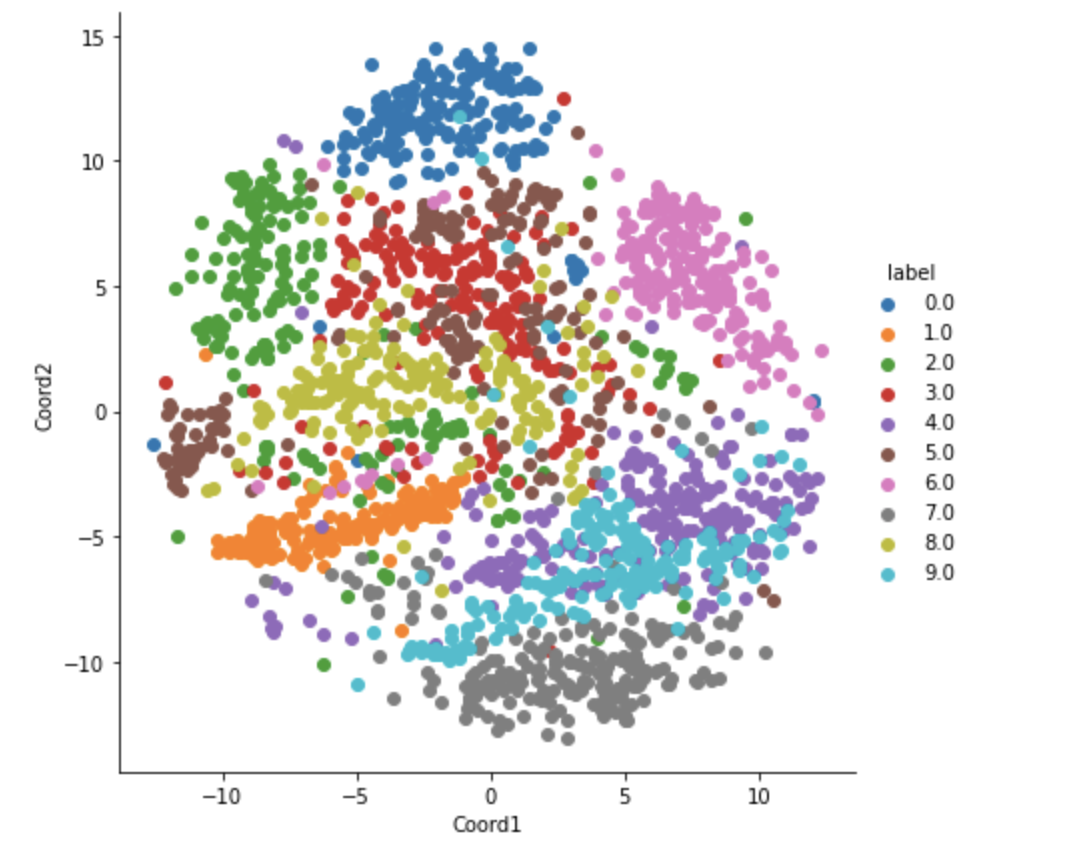
\includegraphics[width=1\textwidth]{tsne-mnist.png}
\end{figure}

For the most part, t-SNE does a good job of separating out the clusters present in the MNIST data. There is some mixing across a few classes; however, the majority of classes are indeed separated into their own clusters, and it is relatively easy to distinguish between classes visually.

\newpage
\subsection*{Olivetti Faces Dataset}

The Olivetti faces dataset consists of images of 40 individuals with small variations in viewpoint, large variations in expression, and the occasional addition of glasses. It consists of 400 images (10 per individual) of size 64x64 = 4,096 pixels, and is labeled according to the identity of the individual. Each image is quantized to 256 grey levels and stored as unsigned 8-bit integers, then converted to floating point values between 0 and 1.

\begin{figure}[H]
\caption{t-SNE on the Olivetti Faces Data set, Labeled}
\centering
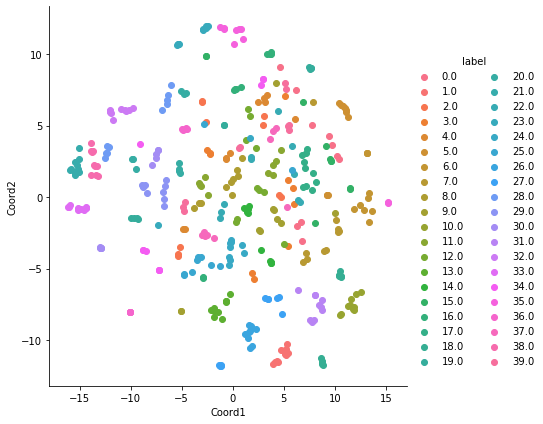
\includegraphics[width=1\textwidth]{tsne-olivetti.png}
\end{figure}

For the Olivetti faces data set, t-SNE again does a pretty good job of revealing the natural classes in the data, with many individuals having relatively distinct clusters. As brought up in the original paper, for those who have their images split into two clusters, this is usually because a subset of their images have the head facing in a significantly different direction, they have a very different expression, or they have glasses on.

\newpage
\subsection*{COIL-20 Data set}

The COIL-20 data set consists of images of 20 different objects viewed from 72 equally spaced orientations, yielding a total of 1,440 images. Each image is of size 32×32 = 1,024 pixels, and labels correspond to each object.

\begin{figure}[H]
\caption{t-SNE on the COIL-20 Data set, Labeled}
\centering
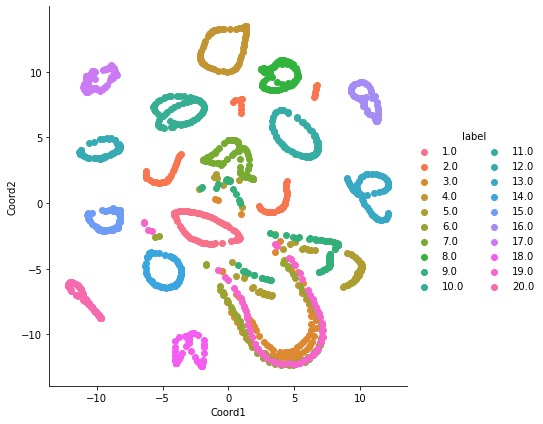
\includegraphics[width=1\textwidth]{tsne-coil20.png}
\end{figure}

For the COIL-20 data set, we can see that t-SNE separates the data into very distinct clusters, with most of the objects being visually represented as a closed loop. As mentioned in the original paper, for objects which look similar from the front and the back, t-SNE distorts the loop so that front and back orientations for each image are mapped to nearby points. Looking at the bottom right corner of the plot, we see that the clusters deviate from this closed loop structure and overlap each other. In fact, these overlapping clusters correspond to the toy cars, each of which had photos taken at the same four orientations. It is due to the similarity between different cars at the same orientation that t-SNE was unable to completely separate these clusters.

\newpage
\subsection*{Iris Data set}

The Iris data set contains 3 classes of 50 instances each, where each class refers to a type of iris plant - Setosa, Versicolour, and Virginica. Attributes for each plant include the sepal length, sepal width, petal length, and petal width, all measured in centimeters. A common issue with this data set is that often only two distinct clusters can be identified, as only one class is linearly separable from the other two.

\begin{figure}[H]
\caption{t-SNE on the Iris Data set, Labeled}
\centering
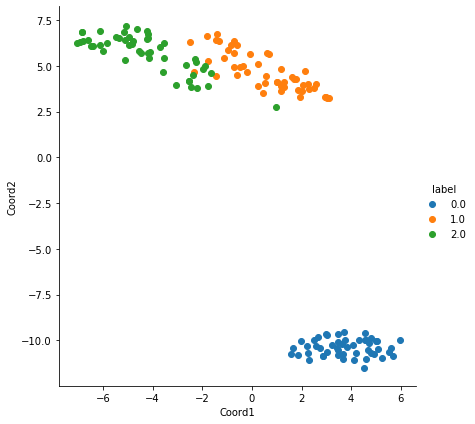
\includegraphics[width=1\textwidth]{tsne-iris.png}
\end{figure}

After applying t-SNE to the Iris data set, we indeed see that one of the classes forms a very distinct cluster from the other two classes. Although the remaining two classes are not as distinctly separated from one another, visually it is still easy to distinguish between the two clusters, and the overlap between the clusters is minimal.

\newpage
\section*{Comparing t-SNE to other algorithms}

\subsection*{PCA}

Principal Components Analysis (PCA) is one of the most widely used dimension reduction methods. The idea of PCA is to reduce the number of variables in a data set while preserving as much information as possible. The first step of PCA involves standardizing the data such that all variables are on the same scale. Next, we must build a $p \times p$ covariance matrix to identify correlations between the different variables. An eigendecomposition is used to identify the principal components, and then a change of basis is employed to recast the data along the principal component axes. Using just the first two principal components, we have a way to visualize high dimensional data on a two dimensional plane. 

Below, we test the use of PCA on the MNIST data set. The PCA recipe we use is implemented with numpy linear algebra operations. The results are shown in Figure 7.

\begin{figure}[H]
\caption{PCA Clustering on the MNIST Dataset, Labeled}
\centering
\includegraphics[width=0.7\textwidth]{pca-mn-col.png}
\end{figure}

In a sense, PCA is able to cluster the data effectively, since dots of the same colors are indeed close to each other on the two dimension projection. However, there is fair amount of mixing between the clusters, making this visualization hard to use. PCA does a very poor job of separating clusters compared to t-SNE. Individual clusters are impossible to ascertain from the PCA visualization. Clearly, PCA is not as useful as t-SNE to visualize this kind of real world data. For dimension reduction tasks other than visualization, PCA may be better than t-SNE since it is much faster and has a elegant mathematical interpretation as well. 

\subsection*{MDS}

While PCA is a popular dimensionality reduction tool, it is not a particularly strong method for visualizing real world data. A method that is designed to visualize the data more effectively is called Multidimensional Scaling, or MDS. Specifically, MDS is designed to visualize the similarity of individual cases in a dataset. In a similar idea to t-SNE, MDS incorporates information about pairwise distances between objects in the data to map them into an abstract cartesian space. Given a distance matrix with the distances between each pair of objects in a set, and a chosen number of dimensions $n$, an MDS algorithm places each object into $n$-dimensional space (a lower-dimensional representation) such that the between-object distances are preserved as well as possible. For low-dimensional $n$, the resulting points can be visualized on a scatter plot. The implementation of MDS we use in this paper comes from sklearn, and the results are shown in Figure 8. 

\begin{figure}[H]
\caption{MDS Clustering on the MNIST Dataset, Labeled}
\centering
\includegraphics[width=0.7\textwidth]{mds-mnist.png}
\end{figure}

MDS does not fare much better than the PCA in terms of producing effective visualizations for the MNIST data. Points of the same colors are close to each other for the most part, but well defined distinct clusters are impossible to ascertain based off of this visualization. t-SNE is clearly superior to both of the tested methods in terms of creating cluster visualizations for real world data. For simulated data, both PCA and MDS often show very strong performance, but real world data is often much more nuanced and requires more sophisticated algorithms to produce well defined clusters in low dimensional visualizations. 

\section*{Discussion and Conclusions}

t-SNE is a particularly strong algorithm for producing striking low dimensional visualizations of data. Compared to many other dimensionality reduction techniques, t-SNE produces visualizations with accurate, well-defined, and well-separated clusters. Because of this, t-SNE can help scientists gain visual insights from their data. t-SNE is very effective, but it can be slow for very large data sets. Creating distance matrices requires many pairwise comparisons, and each gradient step can be expensive to compute. One extension of t-SNE that can increase efficiency avoids computing the gradient step altogether. Instead, optimal $q$ values are found using a method from astrophysics called the Barnes-Hut approximation, which was introduced for the purposes of understanding the motions of clusters of distant planets. Using a quad-tree, an approximate solution to the t-SNE optimization problem can be found in $n \log n$ time, which is must faster than the $n^2$ run time of the classic t-SNE gradient update step. 

One disadvantage to t-SNE is that it is not very useful for dimension reduction tasks outside of visualization, but some novel algorithms are appearing that may outperform t-SNE in many different tasks. A new algorithm for dimensionality reduction that has been developed in the last 5 years is uniform manifold approximation and projection (UMAP). UMAP assumes the data is uniformly distributed on a Riemmanian manifold, which makes the algorithm much more general purpose and flexible than t-SNE. The visualizations UMAP produces are similar to those of t-SNE, but UMAP captures global structure much better than t-SNE does. Finally, much like PCA, UMAP can be used for a much wider range of dimension reduction tasks than t-SNE, such as preprocessing for machine learning. Despite all its advantages, UMAP is new technique, so developed library implementations are hard to come by and best practices are not yet firmly established. 

Despite some of the drawbacks discussed, t-SNE remains a popular and very useful dimensionality reduction algorithm for visualizing data. It is relatively flexible and it can find structures and clusters in data that other algorithms cannot. 
 
\section*{References}

\begin{enumerate}
  \item van der Maaten, Laurens and Hinton, Geoffrey. "Visualizing Data using t-SNE ." Journal of Machine Learning Research 9 (2008): 2579--2605.
  \item https://stackoverflow.com/questions/64952027/compute-l2-distance-with-numpy-using-matrix-multiplication
  \item https://jundongl.github.io/scikit-feature/tutorial.html
  \item https://scikit-learn.org/0.19/datasets/olivetti\_faces.html
\end{enumerate}

\section*{Package Installation}

To install this package, use the following command:
\begin{verbatim}
pip install -i https://test.pypi.org/simple/ tsne-sbmansfield==0.0.1
\end{verbatim}

To use the modules, use the following import command:
\begin{verbatim}
from tsne.tsne import TSNE, plot_tsne
\end{verbatim}

- Refer to examples/tsne-examples.py in the GitHub repository for examples on how to use the TSNE and plot\_tsne functions\\

This process is also outlined in the README of the linked GitHub repository.

\end{document}